\documentclass[11pt, a4paper]{article}

\usepackage[affil-it]{authblk}
\usepackage{etoolbox}
\usepackage{lmodern}
\usepackage{titlesec}
\usepackage{float}
\usepackage{amsfonts}
\usepackage{hyperref}
\usepackage{listings}
\usepackage{color}
\usepackage{graphicx}
\usepackage{subcaption}
\usepackage{amsmath}
\usepackage{relsize}
\usepackage[a4paper, margin=1in]{geometry}

\makeatletter
\patchcmd{\@maketitle}{\LARGE \@title}{\fontsize{20}{19.2}\selectfont\@title}{}{}
\makeatother

\renewcommand\Authfont{\fontsize{16}{14.4}\selectfont}
\renewcommand\Affilfont{\fontsize{12}{10.8}\itshape}

\title{\textbf{AE 706: Assignment 4}}
\author{Pavan R Hebbar - 130010046}

\definecolor{codegreen}{rgb}{0,0.6,0}
\definecolor{codegray}{rgb}{0.5,0.5,0.5}
\definecolor{codepurple}{rgb}{0.58,0,0.82}
\definecolor{backcolour}{rgb}{0.95,0.95,0.92}
 
\lstdefinestyle{mystyle}{
    backgroundcolor=\color{backcolour},   
    commentstyle=\color{codegreen},
    keywordstyle=\color{magenta},
    numberstyle=\tiny\color{codegray},
    stringstyle=\color{codepurple},
    basicstyle=\footnotesize,
    breakatwhitespace=false,         
    breaklines=true,                 
    captionpos=b,                    
    keepspaces=true,                 
    numbers=left,                    
    numbersep=5pt,                  
    showspaces=false,                
    showstringspaces=false,
    showtabs=false,                  
    tabsize=2
}
\lstset{style=mystyle}

\begin{document}
\maketitle
\newpage
\tableofcontents
\newpage
\section{Introduction:}
This assignment deals with the implementation of FTCS and Lax Friedrichs scheme. We solve two problems - one, dealing with the
flow from a high pressure reservoir to ambient atmosphere through a pipe and second dealing with shock tube.

\section{Question 1:}
In this question we implement the FTCS scheme along with some articial dissipation to make the scheme stable. i.e the following
is followed:
\begin{equation}
 Q_p^{q+1} = Q_{p}^{q+1} - \frac{\Delta t}{\Delta x}\left[E_{p+1}^{q} - E_{p-1}^q\right] + \mu_2\frac{\partial^2 Q}{\partial x^2}
 + \mu_4\frac{\partial^4 Q}{\partial x^4}
\end{equation}
We take $\mu_2 = 0.01$ and $\mu_4 = 0.001$. The second derivative term with positive $\mu_2$ makes the scheme stable and
prevents the divergence of the scheme. The fourth derivative term with positive $\mu_4$ is used to reduce the dissipation of 
higher wave numbers, so that the solution doesn't smoothen out. We use central difference to evaluate the second derivative.
Since the central difference for a fourth order derivative requires two neighbouring points on each side, we use forward 
difference to evaluate the $4^th$ order derivative at $1^st$ and backward difference last grid points and central difference for rest of the 
points (All finite difference schemes of 2nd order accuracy). This question deals with testing our code for standard case. Following boundary conditions were used
\begin{itemize}
 \item \textbf{Inlet}: $P_0 = 101325$ Pa, $T_0 = 300K$
 \item \textbf{Outlet}: $P_a = 84000$ Pa
\end{itemize}
Initially the region was set to outlet conditions so that the wave propogates from the reservoir to exit (left to right) with
ambient temperature $T_a = 300K$. Note that $T_a$ doesn't change the physics of the problem but is requred for the
implementation of the schemes.
The length of the pipe was taken to me 1 (normalised units). The domain was divided into 1000 grid points so that 
$\Delta x = 0.001$. Then the simulation was run for $\Delta t = 0.0001\Delta x, 0.0003\Delta x, 0.0004\Delta x)$.
The simulation was performed for 

\subsection{Case 1: $\Delta t = 0.0001\Delta x$}:
Under this choice of $\Delta t$, we see that the scheme is stable and shows the propogation of waves. Following are the variation
of density, velocity and pressure wrt x at different times (till $0.003s$):
\begin{figure}[H]
 \centering
 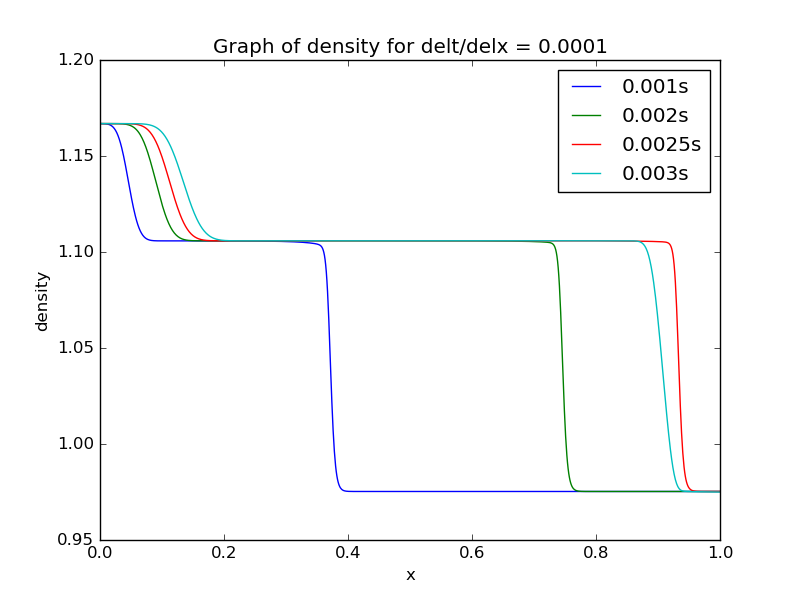
\includegraphics[width = 0.9\textwidth]{FTCS2_1_1.png}
 \caption{Plot of density v/s x}
\end{figure}
\begin{figure}[H]
 \centering
 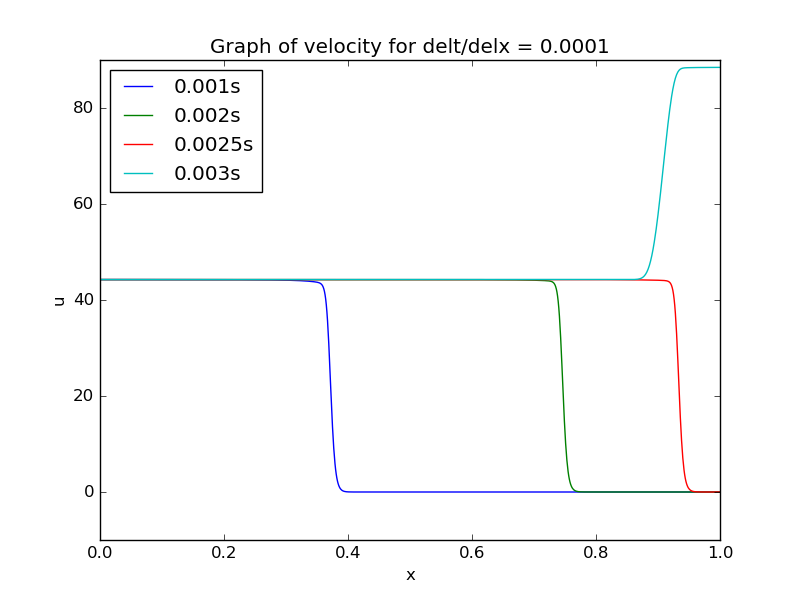
\includegraphics[width = 0.9\textwidth]{FTCS2_1_4.png}
 \caption{Plot of velocity v/s x}
\end{figure}
\begin{figure}[H]
 \centering
 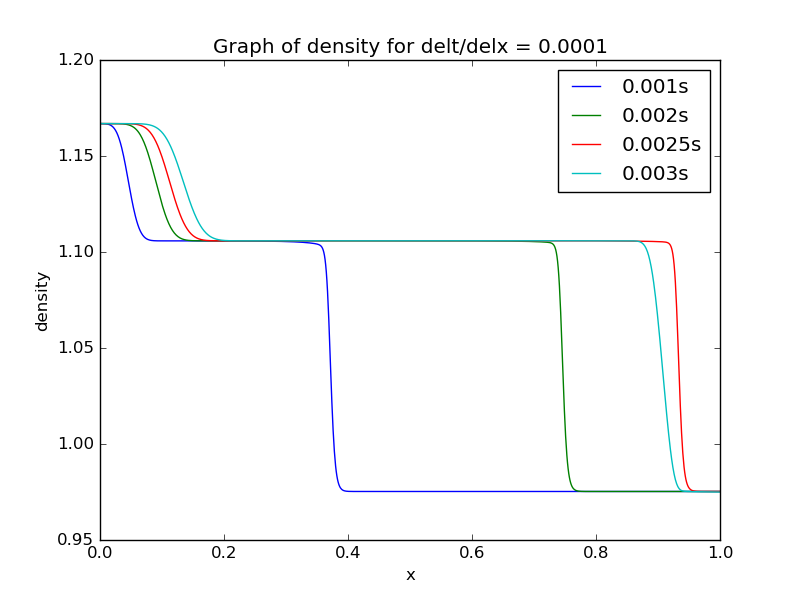
\includegraphics[width = 0.9\textwidth]{FTCS2_1_1.png}
 \caption{Plot of pressure v/s x}
\end{figure}

On analysing the density plot we can see that the density is being propogated by two waves. On comparing with the velocity plot,
we can see that the speed of propogation of one of the waves is equal to $u$ and that of the other wave is $u + c$. Pressure and
velocity are propogated only by one wave corresponding to speed $u+c$. We see
that at $0.003s$, the wave has already been reflected from the wall. We also see that both $u$ and $P$ are being propogated 
with a velocity of $u+c$. The sudden changes in the $\rho$, $p$, $u$ due to the faster wave show that it is a shock.
The subsequent variation of these properties from $0.003$ to $0.006$ is shown below:
\begin{figure}[H]
 \centering
 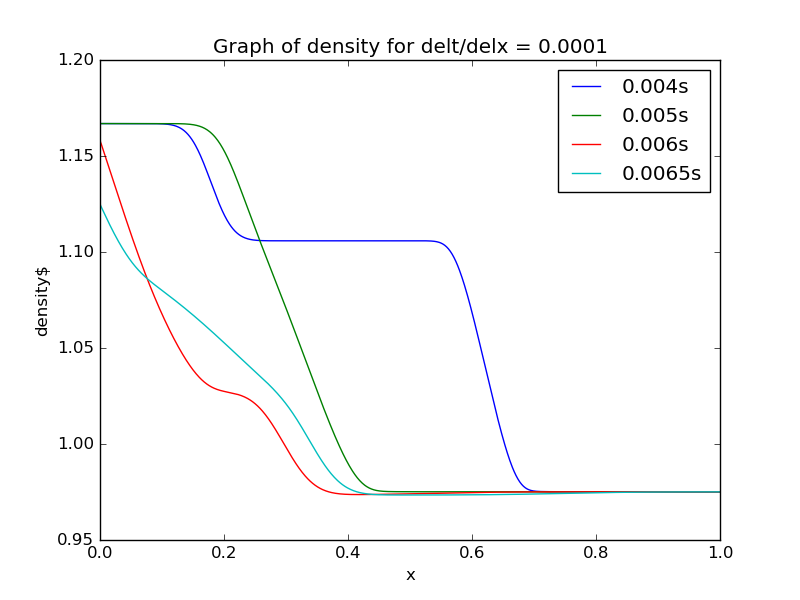
\includegraphics[width = 0.9\textwidth]{FTCS2_1_2.png}
 \caption{Plot of density v/s x}
\end{figure}
\begin{figure}[H]
 \centering
 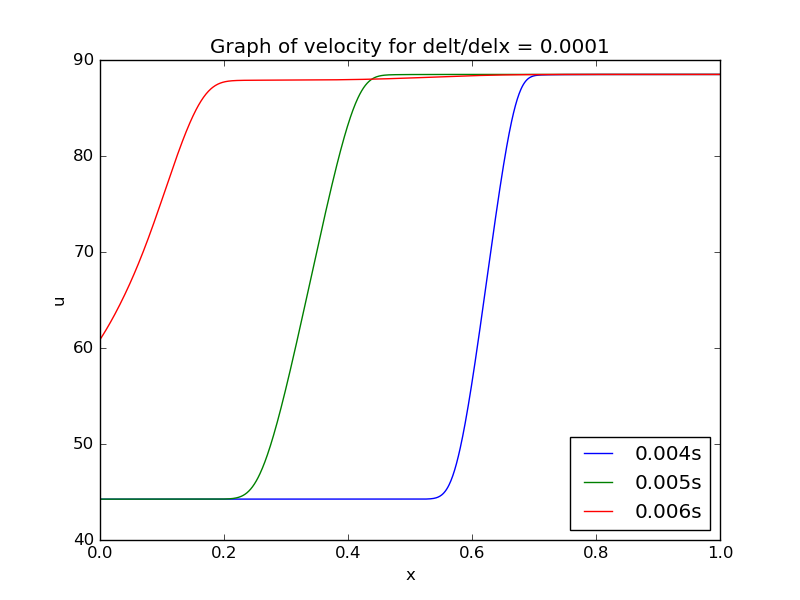
\includegraphics[width = 0.9\textwidth]{FTCS2_1_5.png}
 \caption{Plot of velocity v/s x}
\end{figure}
\begin{figure}[H]
 \centering
 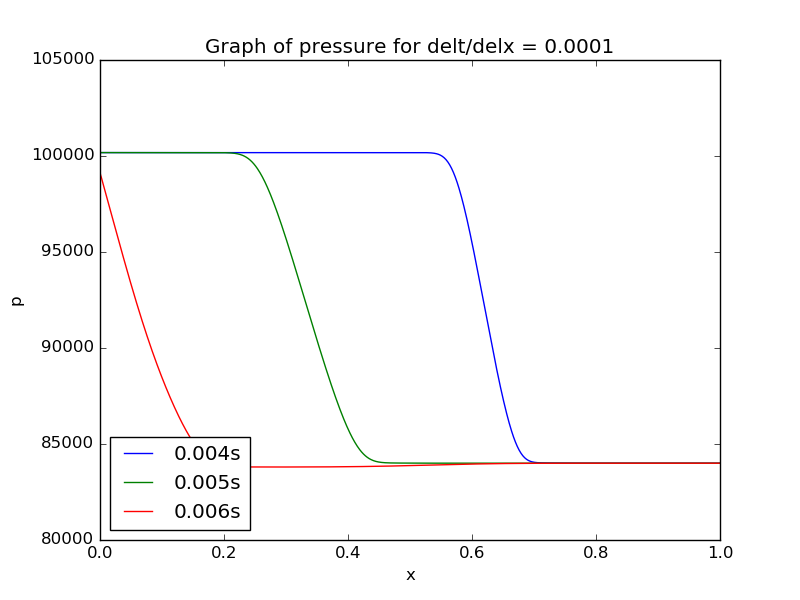
\includegraphics[width = 0.9\textwidth]{FTCS2_1_8.png}
 \caption{Plot of pressure v/s x}
\end{figure}

These plots show the propogation of the waves after being reflected from the outlet. The gradual change in the properties 
across this wave indicates thas the reflected wave is an expansion fan. Also the speed of this expansion fan is slower in 
comparision to the one before reflection. This is because since u is positive, the speed of the characteristics from left to 
right has to be $u-c$. Note that the velocity increases across this expansion fan. at $t = 0.005s$ we see that the 2 waves 
overlap, but from the plot at $t=0.006s$, we can see that these waves propogate as if they were undisturbed. It can also be 
noted the the speed of propogation of the wave from left the right roubly doubles after this. This is due to the increase in 
$u$ downstream of the expansion fan.

Subsequent variation in the properties after $t=0.006$ are shown below.
\begin{figure}[H]
 \centering
 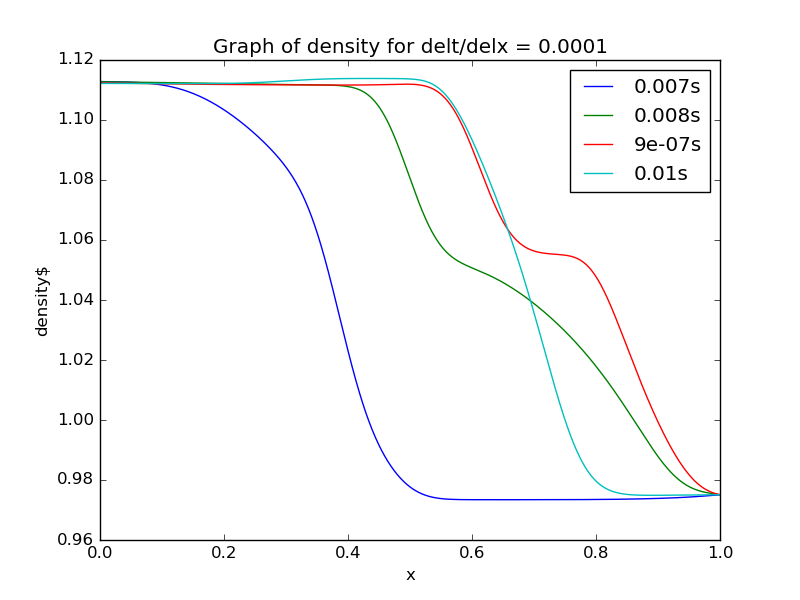
\includegraphics[width = 0.9\textwidth]{FTCS2_1_3.png}
 \caption{Plot of density v/s x}
\end{figure}
\begin{figure}[H]
 \centering
 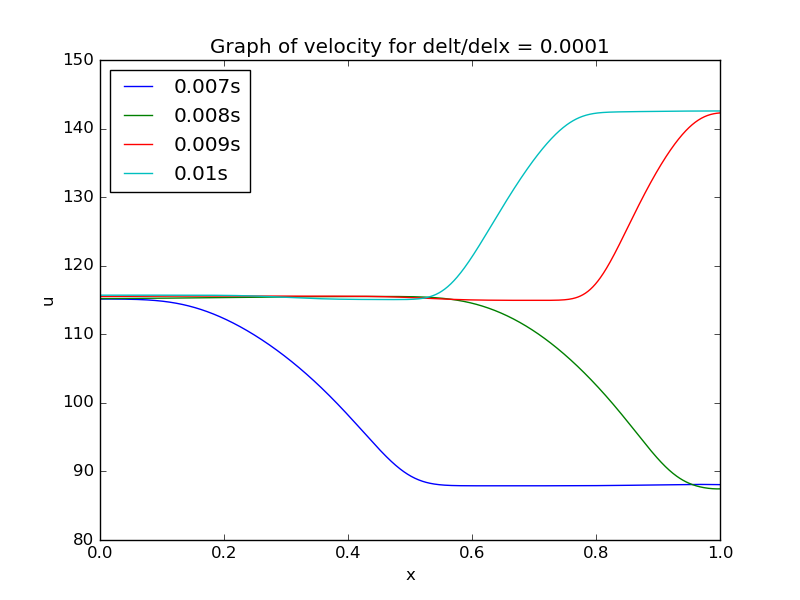
\includegraphics[width = 0.9\textwidth]{FTCS2_1_6.png}
 \caption{Plot of velocity v/s x}
\end{figure}
\begin{figure}[H]
 \centering
 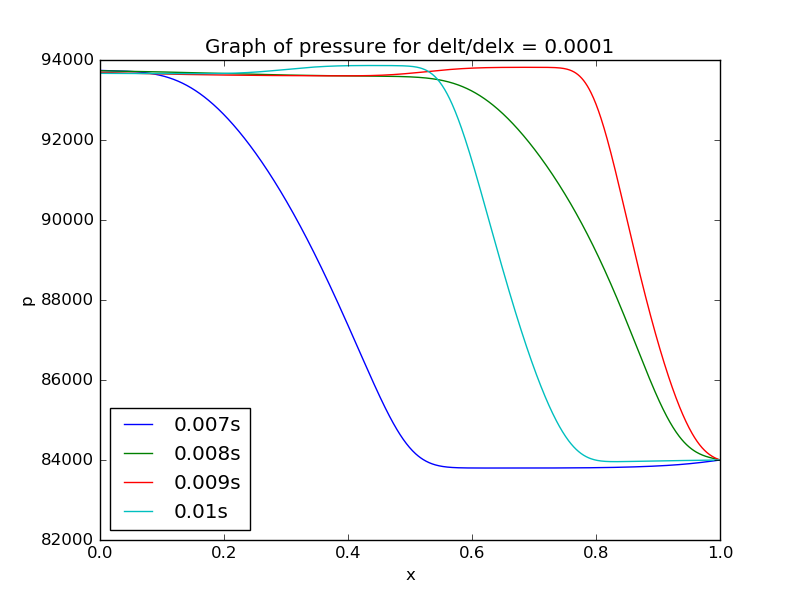
\includegraphics[width = 0.9\textwidth]{FTCS2_1_9.png}
 \caption{Plot of pressure v/s x}
\end{figure}

These plots agree with the previous conclusions regarding the speed of the propogating waves. At the same time we can see that 
the jump in the quantities across the wave decreases after each reflection indicating that a steady state shall be achieved in
due time.

\subsection{Case 2: $\Delta t = 0.0003 \Delta x$}

All results are same as above except that there is an increased amplitude of higher order terms. The amplitude of these 
oscillations doesn't increase with time. This implies that this is probably the result of some left over negative dissipation
and some amount of dispersion. We also see that the graphs are sharper as compared to the previous case implying that that
there is less dissipation are shown below

\begin{figure}[H]
 \centering
 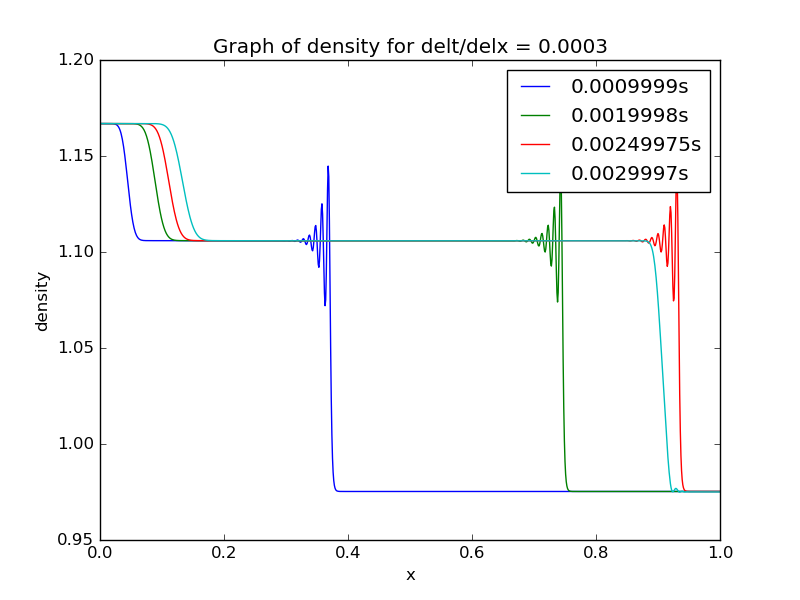
\includegraphics[width = 0.9\textwidth]{FTCS2_2_1.png}
 \caption{Plot of density v/s x}
\end{figure}
\begin{figure}[H]
 \centering
 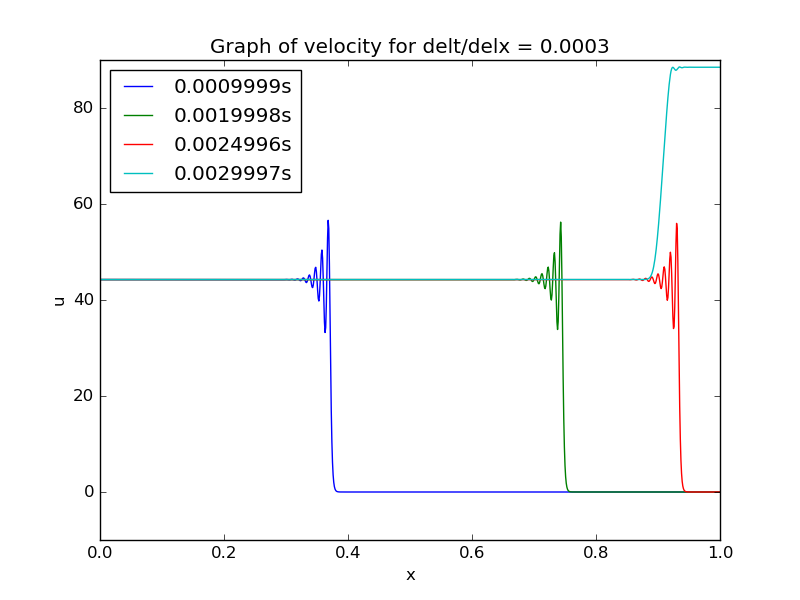
\includegraphics[width = 0.9\textwidth]{FTCS2_2_4.png}
 \caption{Plot of velocity v/s x}
\end{figure}
\begin{figure}[H]
 \centering
 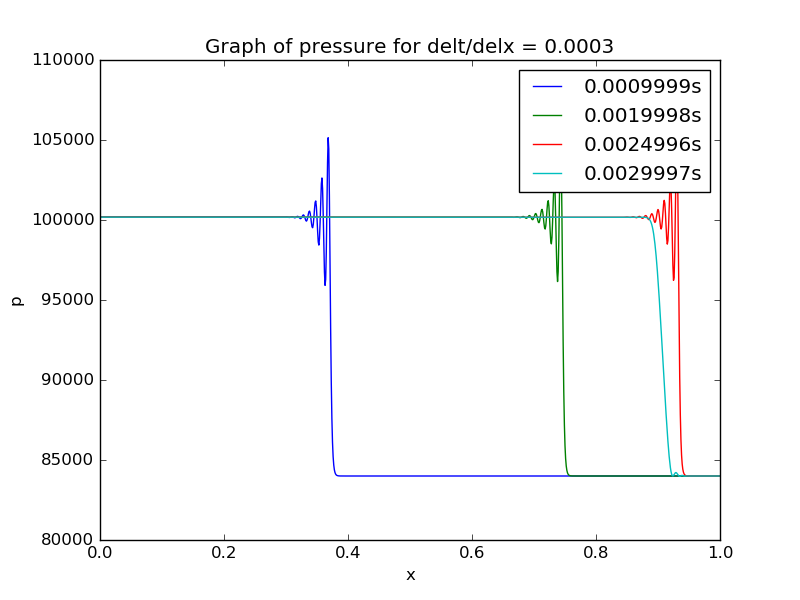
\includegraphics[width = 0.9\textwidth]{FTCS2_2_7.png}
 \caption{Plot of pressure v/s x}
\end{figure}
\begin{figure}[H]
 \centering
 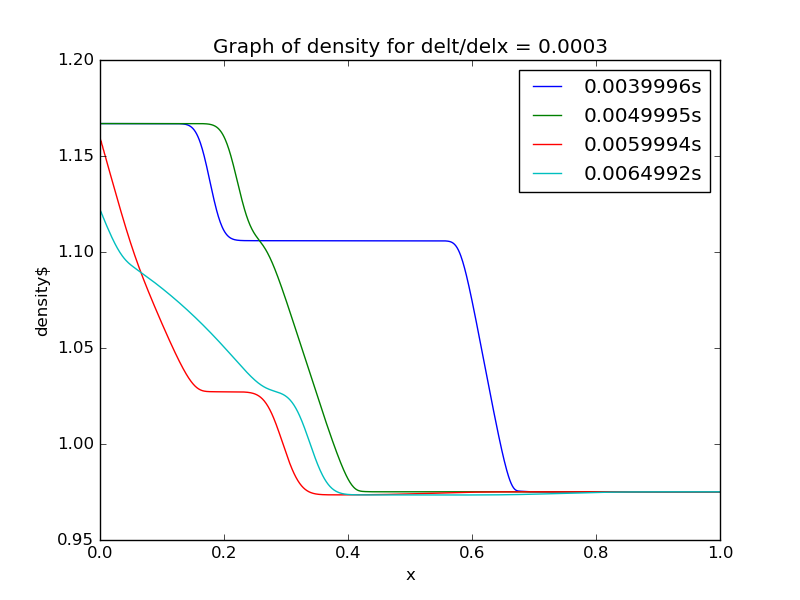
\includegraphics[width = 0.9\textwidth]{FTCS2_2_2.png}
 \caption{Plot of density v/s x}
\end{figure}
\begin{figure}[H]
 \centering
 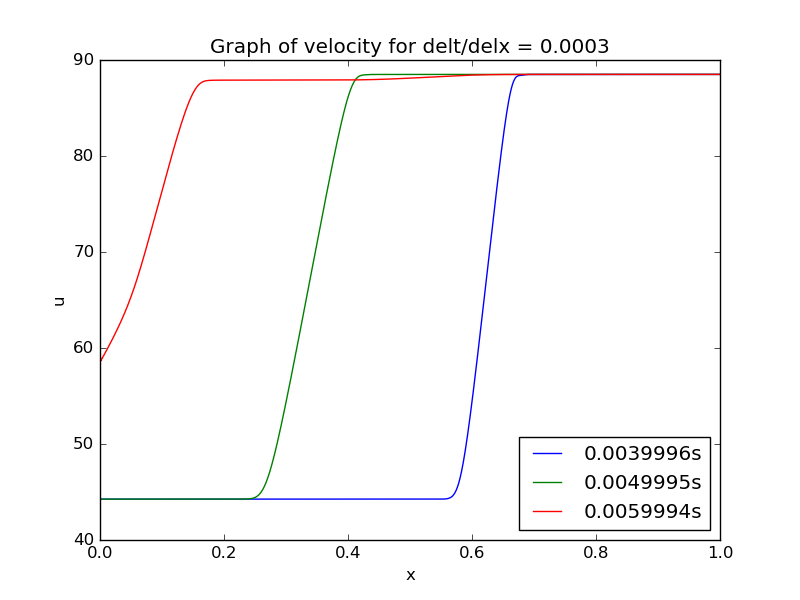
\includegraphics[width = 0.9\textwidth]{FTCS2_2_5.png}
 \caption{Plot of velocity v/s x}
\end{figure}
\begin{figure}[H]
 \centering
 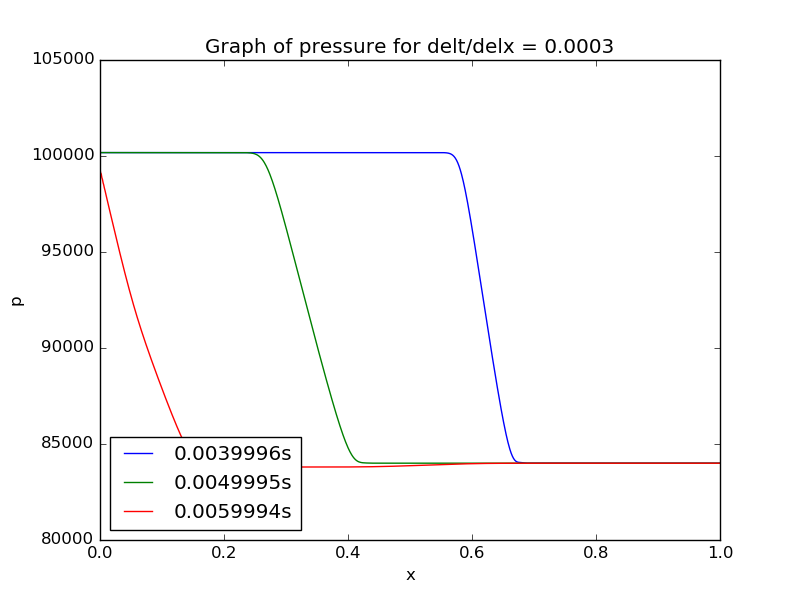
\includegraphics[width = 0.9\textwidth]{FTCS2_2_8.png}
 \caption{Plot of pressure v/s x}
\end{figure}
\begin{figure}[H]
 \centering
 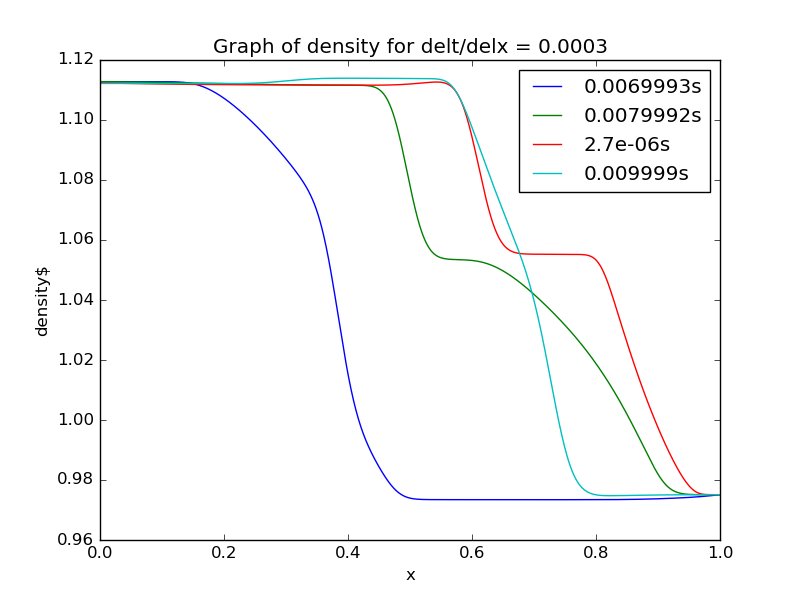
\includegraphics[width = 0.9\textwidth]{FTCS2_2_3.png}
 \caption{Plot of density v/s x}
\end{figure}
\begin{figure}[H]
 \centering
 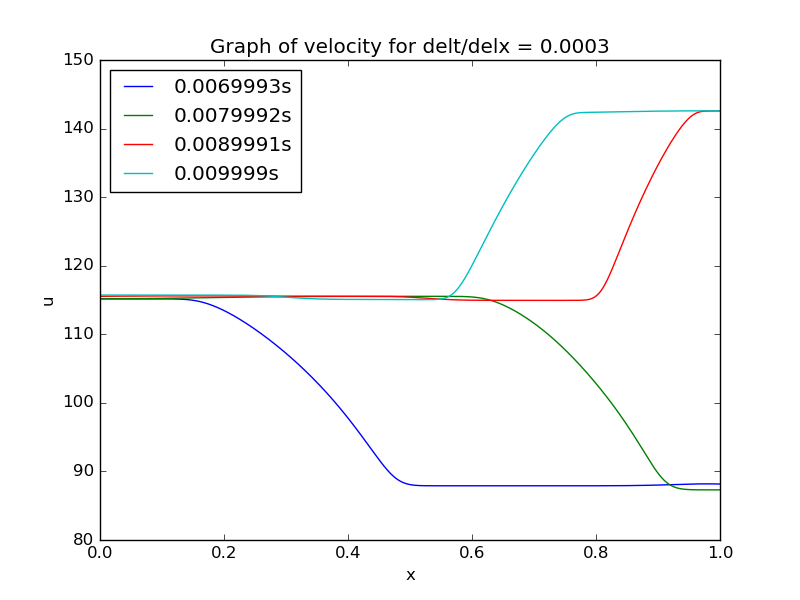
\includegraphics[width = 0.9\textwidth]{FTCS2_2_6.png}
 \caption{Plot of velocity v/s x}
\end{figure}
\begin{figure}[H]
 \centering
 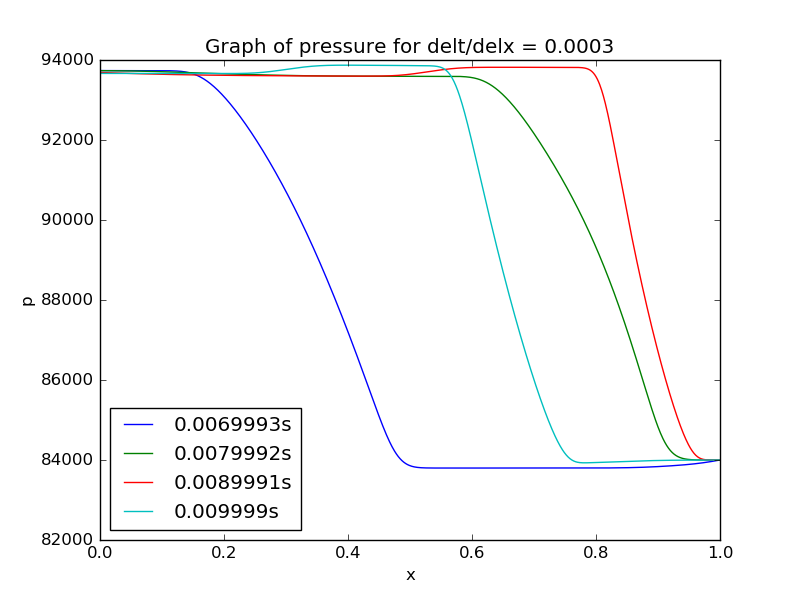
\includegraphics[width = 0.9\textwidth]{FTCS2_2_9.png}
 \caption{Plot of pressure v/s x}
\end{figure}

\subsection{Case 3: $\Delta t = 0.0004 \Delta x$}

We see that the scheme is unstable under this choice of $\Delta t$. This can be seen by the increasing amplitude of oscillations
\begin{figure}[H]
 \centering
 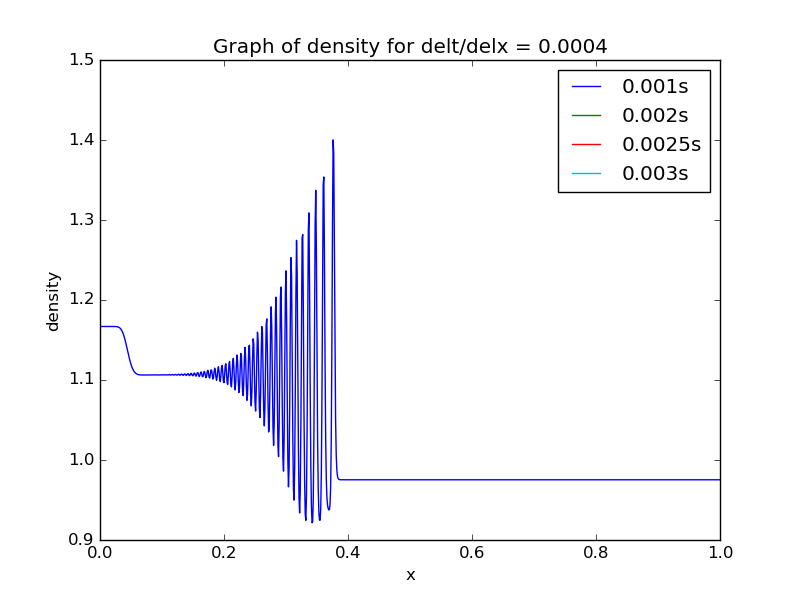
\includegraphics[width = 0.9\textwidth]{FTCS2_3_1.png}
 \caption{Plot of density v/s x}
\end{figure}
\begin{figure}[H]
 \centering
 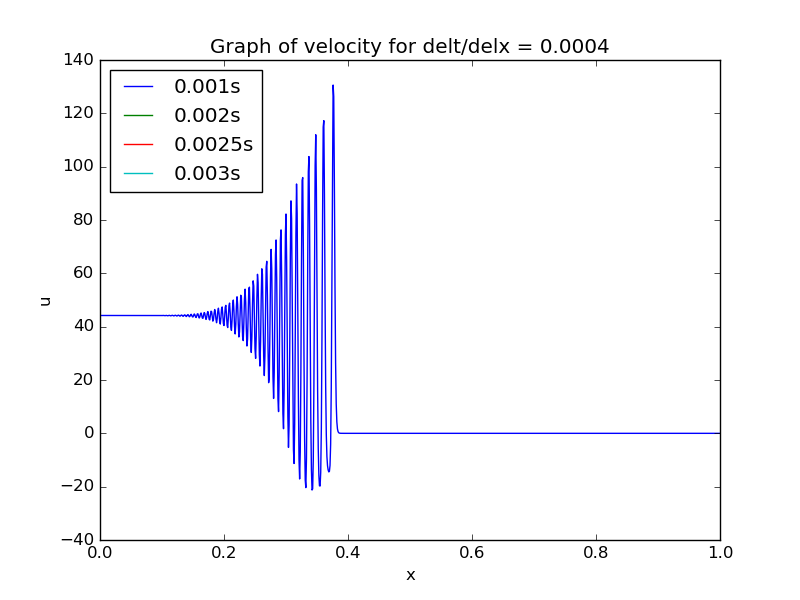
\includegraphics[width = 0.9\textwidth]{FTCS2_3_4.png}
 \caption{Plot of velocity v/s x}
\end{figure}
\begin{figure}[H]
 \centering
 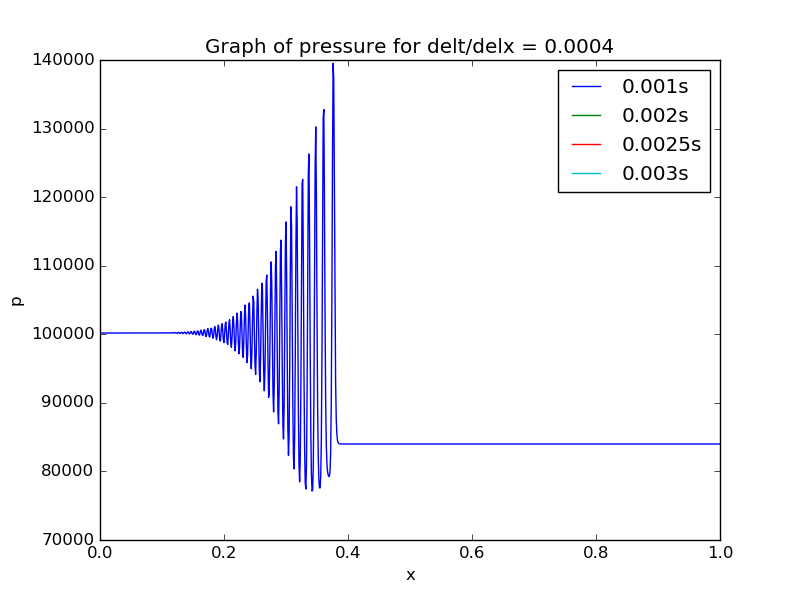
\includegraphics[width = 0.9\textwidth]{FTCS2_3_7.png}
 \caption{Plot of pressure v/s x}
\end{figure}

\section{Question 2}:
In this question we solve the same problem with Lax-Friedrichs scheme. We see that the scheme is more stable in FTCS but
it smoothens the waves a lot. Increasing the ratio of $\Delta t/\Delta x$ sharpens the solution but it is still
smooth as compared to FTCS. Below are the plots obtained:
\subsection{Case 1: $\Delta t = 0.0001 \Delta x$}
\begin{figure}[H]
 \centering
 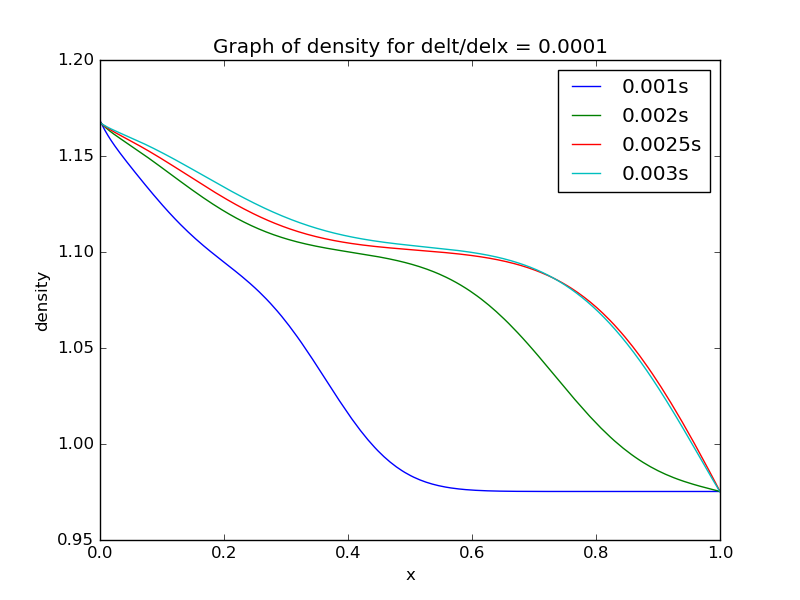
\includegraphics[width = 0.9\textwidth]{lax_fed_1_1.png}
 \caption{Plot of density v/s x}
\end{figure}
\begin{figure}[H]
 \centering
 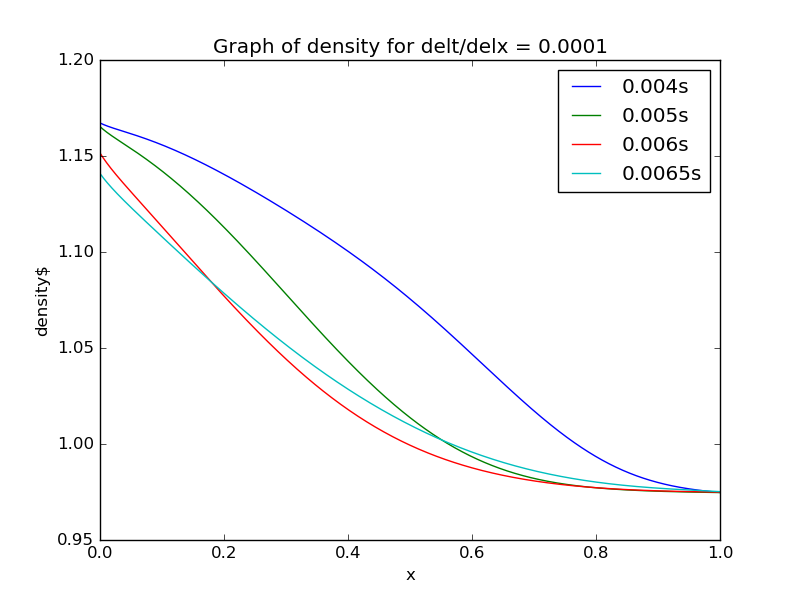
\includegraphics[width = 0.9\textwidth]{lax_fed_1_2.png}
 \caption{Plot of density v/s x}
\end{figure}
\begin{figure}[H]
 \centering
 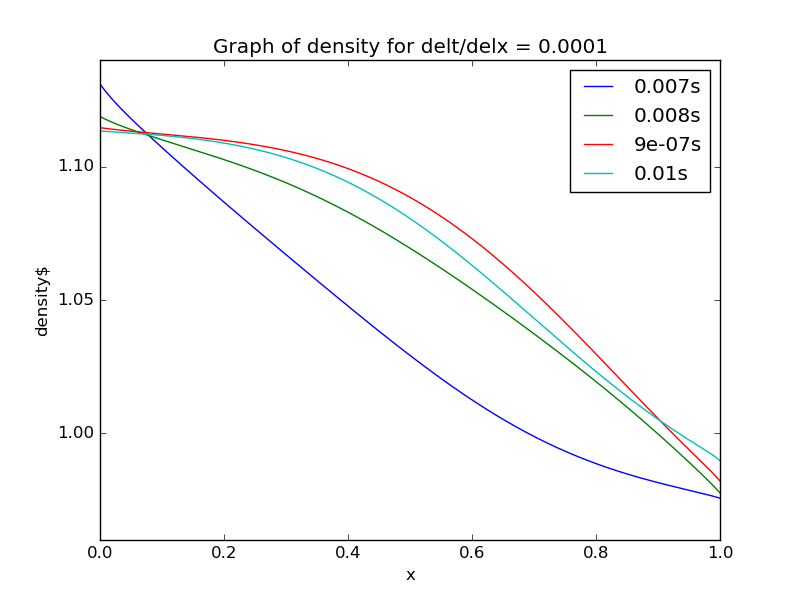
\includegraphics[width = 0.9\textwidth]{lax_fed_1_3.png}
 \caption{Plot of density v/s x}
\end{figure}
\begin{figure}[H]
 \centering
 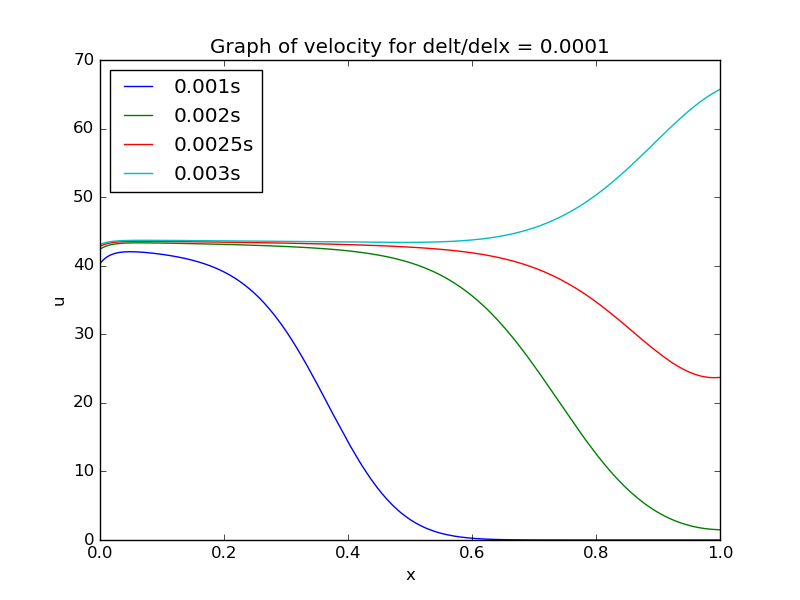
\includegraphics[width = 0.9\textwidth]{lax_fed_1_4.png}
 \caption{Plot of velocity v/s x}
\end{figure}
\begin{figure}[H]
 \centering
 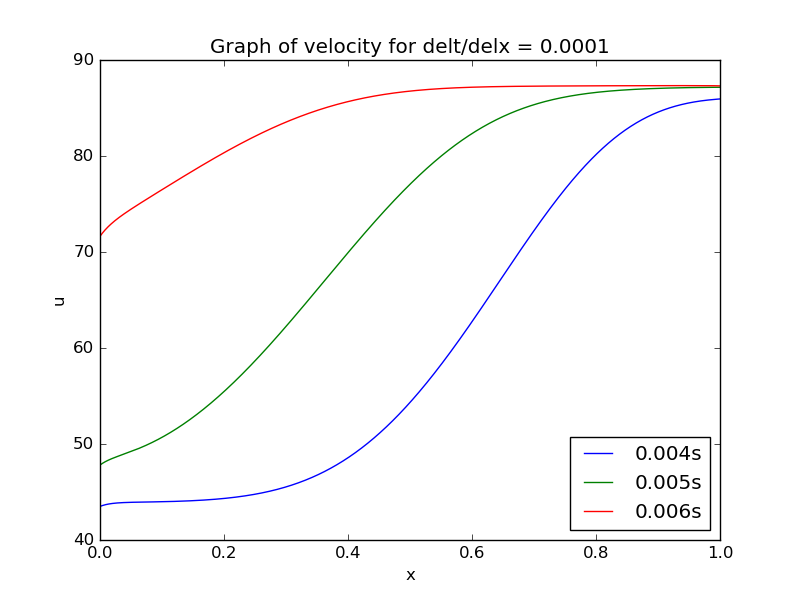
\includegraphics[width = 0.9\textwidth]{lax_fed_1_5.png}
 \caption{Plot of velocity v/s x}
\end{figure}
\begin{figure}[H]
 \centering
 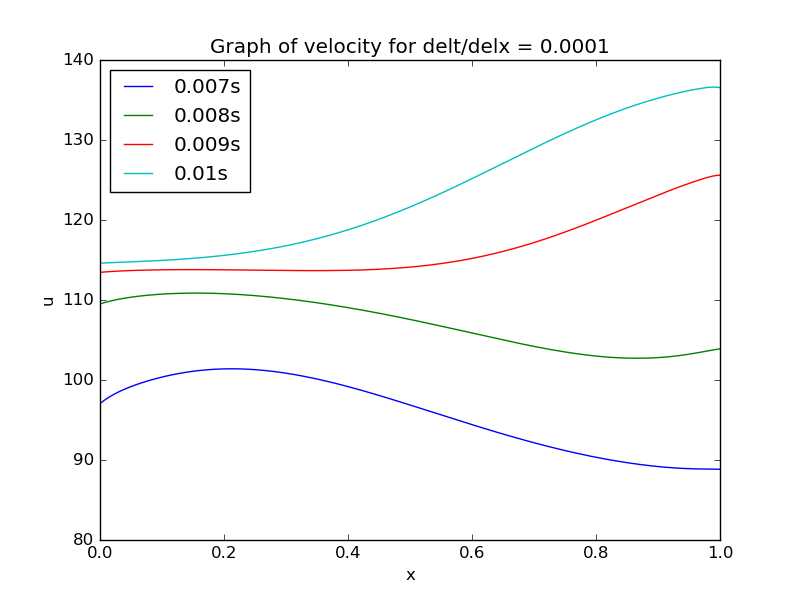
\includegraphics[width = 0.9\textwidth]{lax_fed_1_6.png}
 \caption{Plot of velocity v/s x}
\end{figure}
\begin{figure}[H]
 \centering
 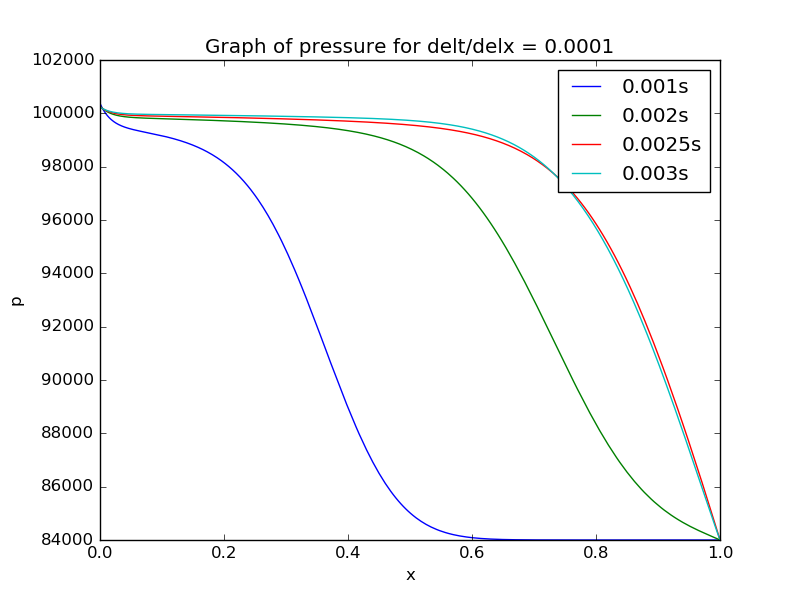
\includegraphics[width = 0.9\textwidth]{lax_fed_1_7.png}
 \caption{Plot of pressure v/s x}
\end{figure}
\begin{figure}[H]
 \centering
 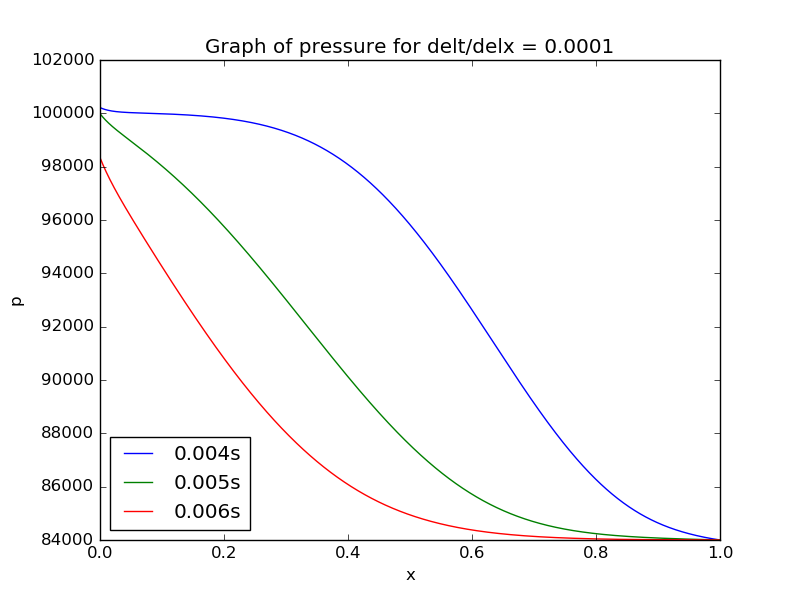
\includegraphics[width = 0.9\textwidth]{lax_fed_1_8.png}
 \caption{Plot of pressure v/s x}
\end{figure}
\begin{figure}[H]
 \centering
 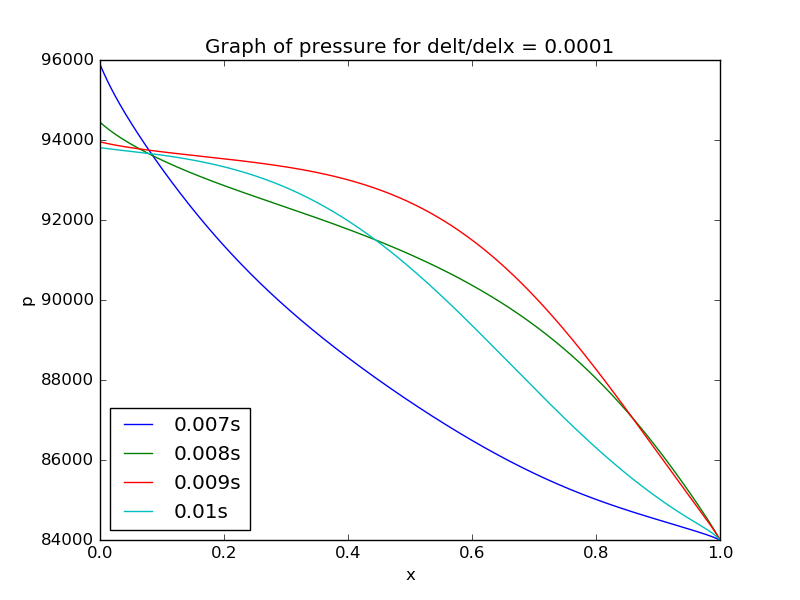
\includegraphics[width = 0.9\textwidth]{lax_fed_1_9.png}
 \caption{Plot of pressure v/s x}
\end{figure}

\subsection{Case 2: $\Delta t = 0.0005 \Delta x$}
\begin{figure}[H]
 \centering
 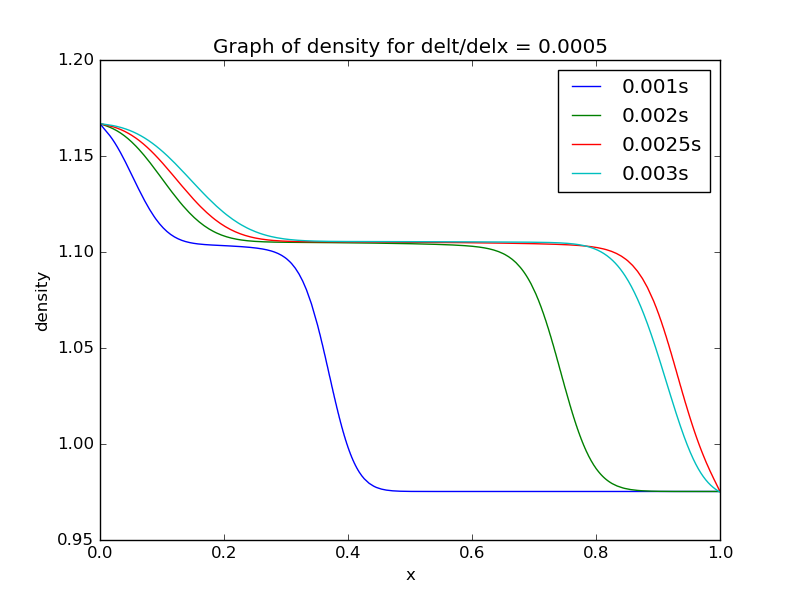
\includegraphics[width = 0.9\textwidth]{lax_fed_2_1.png}
 \caption{Plot of density v/s x}
\end{figure}
\begin{figure}[H]
 \centering
 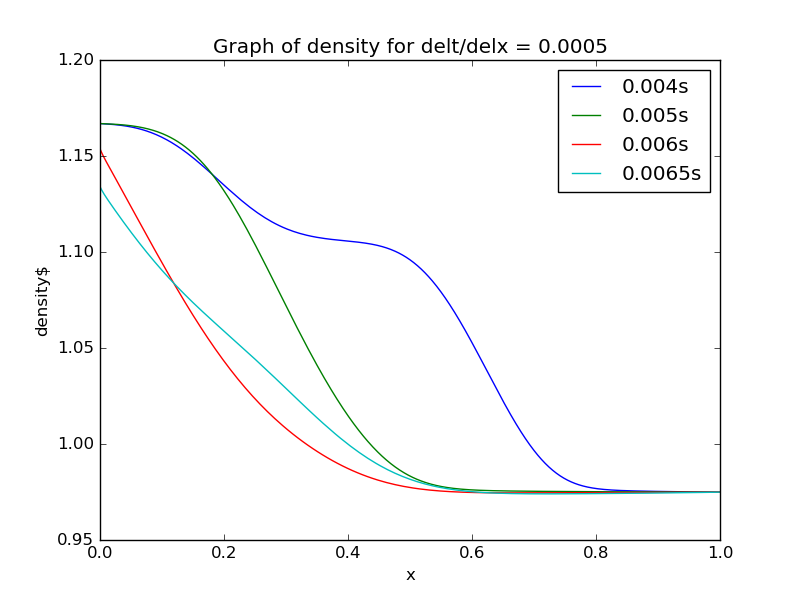
\includegraphics[width = 0.9\textwidth]{lax_fed_2_2.png}
 \caption{Plot of density v/s x}
\end{figure}
\begin{figure}[H]
 \centering
 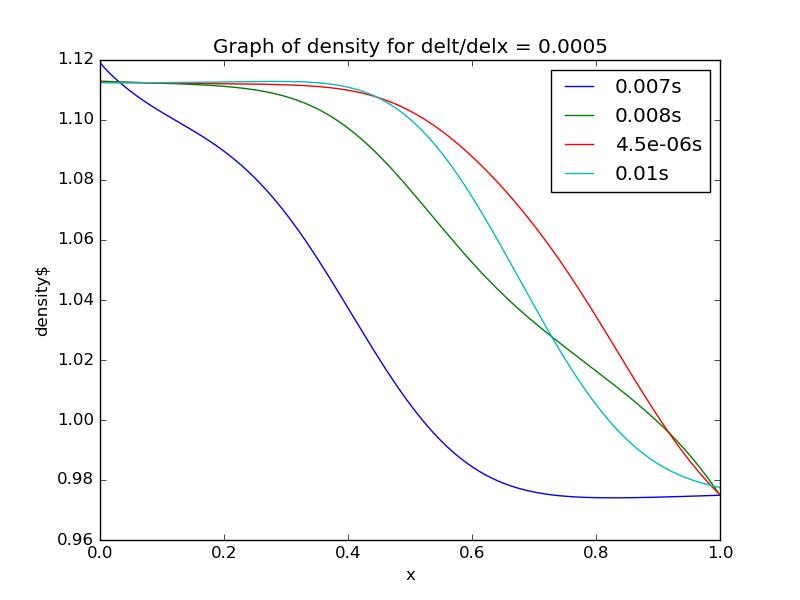
\includegraphics[width = 0.9\textwidth]{lax_fed_2_3.png}
 \caption{Plot of density v/s x}
\end{figure}
\begin{figure}[H]
 \centering
 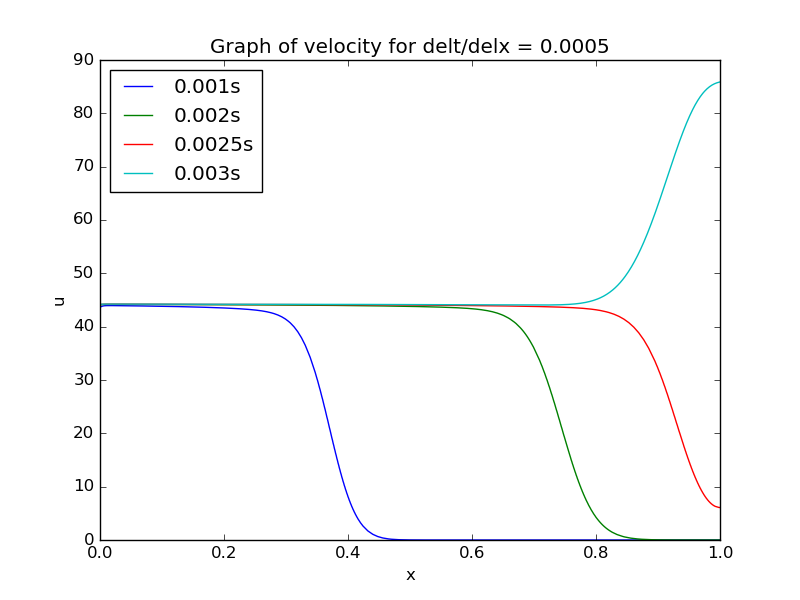
\includegraphics[width = 0.9\textwidth]{lax_fed_2_4.png}
 \caption{Plot of velocity v/s x}
\end{figure}
\begin{figure}[H]
 \centering
 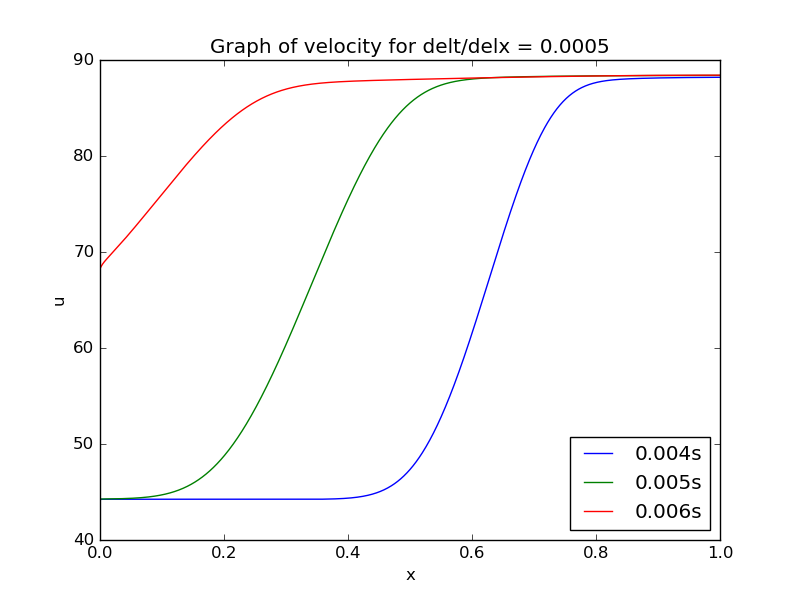
\includegraphics[width = 0.9\textwidth]{lax_fed_2_5.png}
 \caption{Plot of velocity v/s x}
\end{figure}
\begin{figure}[H]
 \centering
 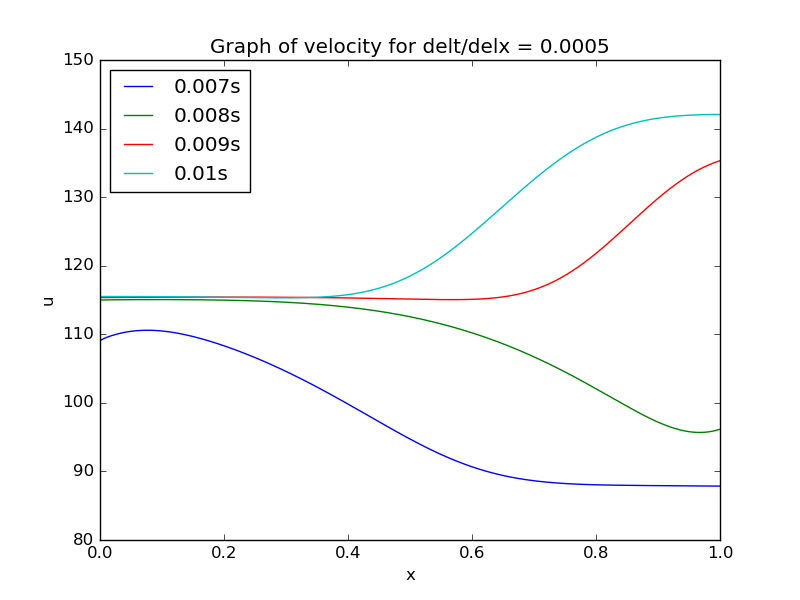
\includegraphics[width = 0.9\textwidth]{lax_fed_2_6.png}
 \caption{Plot of velocity v/s x}
\end{figure}
\begin{figure}[H]
 \centering
 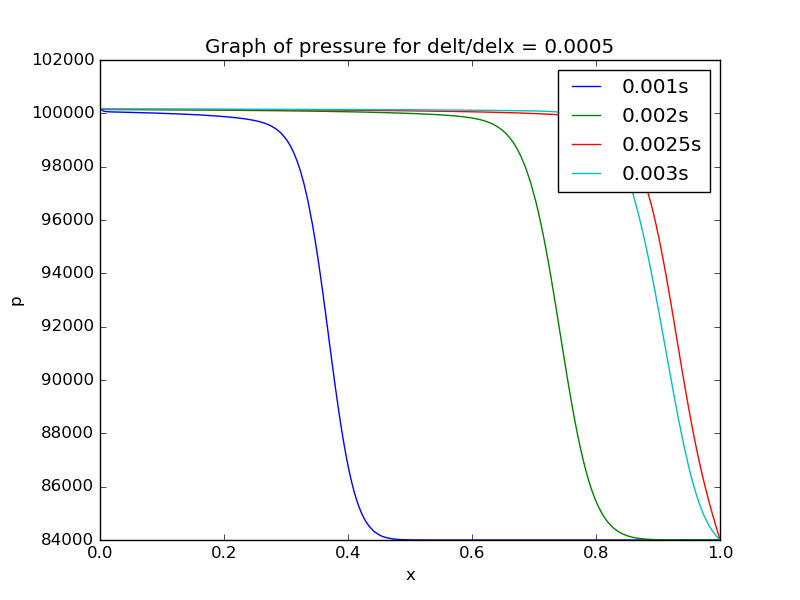
\includegraphics[width = 0.9\textwidth]{lax_fed_2_7.png}
 \caption{Plot of pressure v/s x}
\end{figure}
\begin{figure}[H]
 \centering
 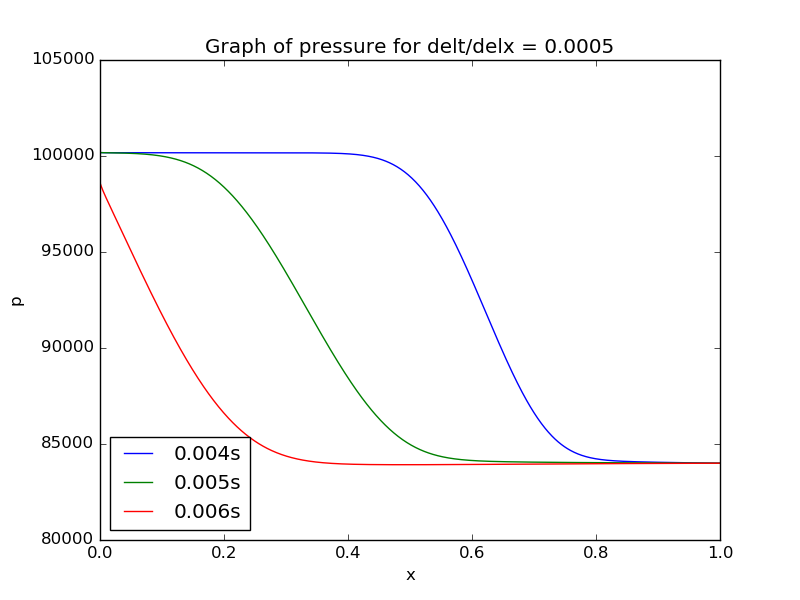
\includegraphics[width = 0.9\textwidth]{lax_fed_2_8.png}
 \caption{Plot of pressure v/s x}
\end{figure}
\begin{figure}[H]
 \centering
 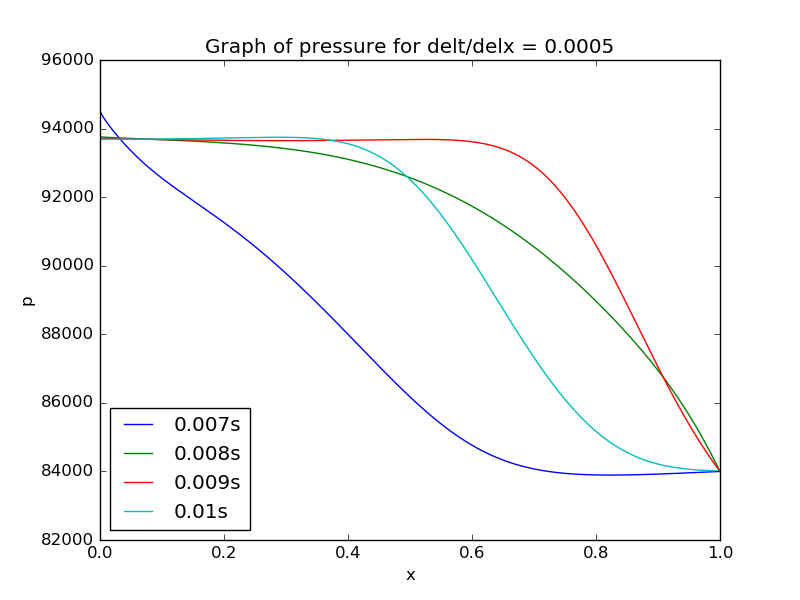
\includegraphics[width = 0.9\textwidth]{lax_fed_2_9.png}
 \caption{Plot of pressure v/s x}
\end{figure}

\subsection{Case 2: $\Delta t = 0.001 \Delta x$}
\begin{figure}[H]
 \centering
 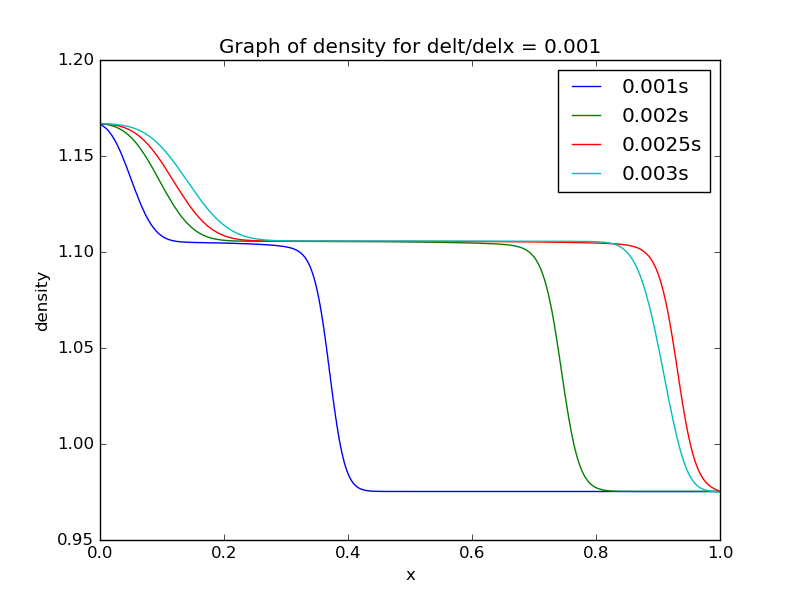
\includegraphics[width = 0.9\textwidth]{lax_fed_3_1.png}
 \caption{Plot of density v/s x}
\end{figure}
\begin{figure}[H]
 \centering
 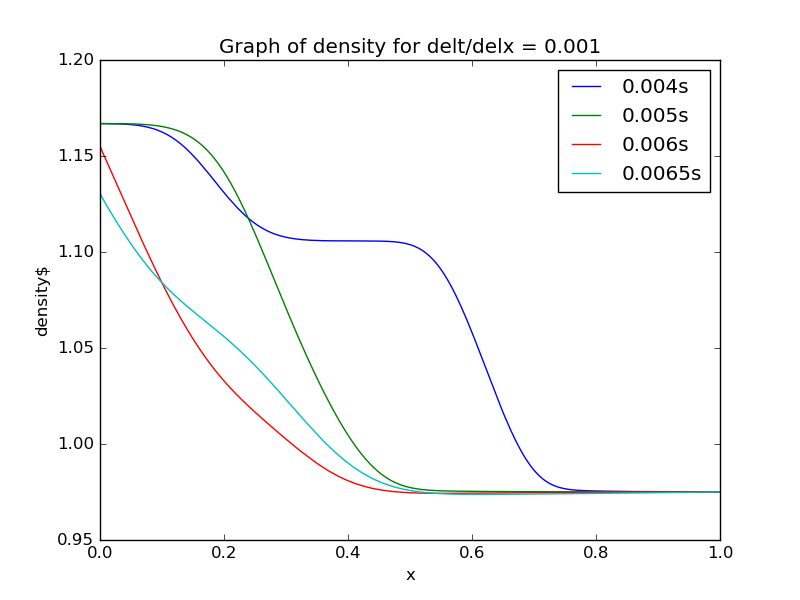
\includegraphics[width = 0.9\textwidth]{lax_fed_3_2.png}
 \caption{Plot of density v/s x}
\end{figure}
\begin{figure}[H]
 \centering
 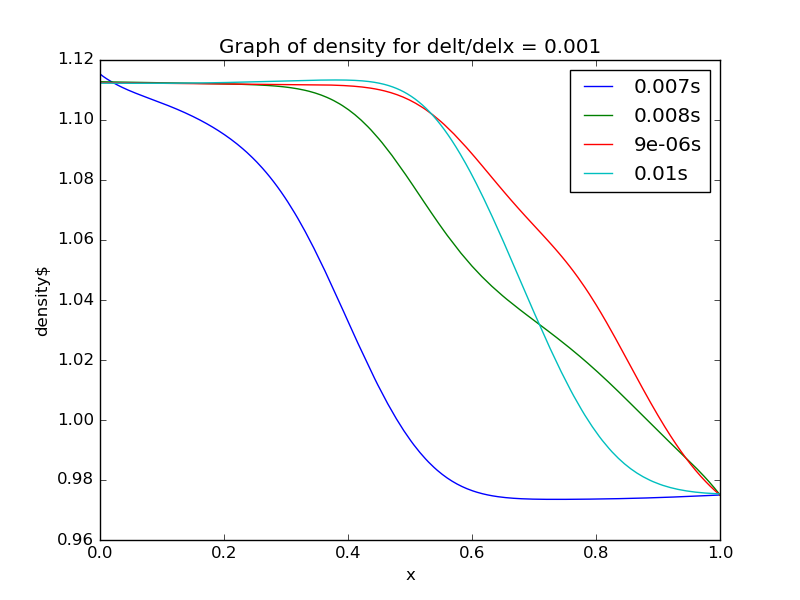
\includegraphics[width = 0.9\textwidth]{lax_fed_3_3.png}
 \caption{Plot of density v/s x}
\end{figure}
\begin{figure}[H]
 \centering
 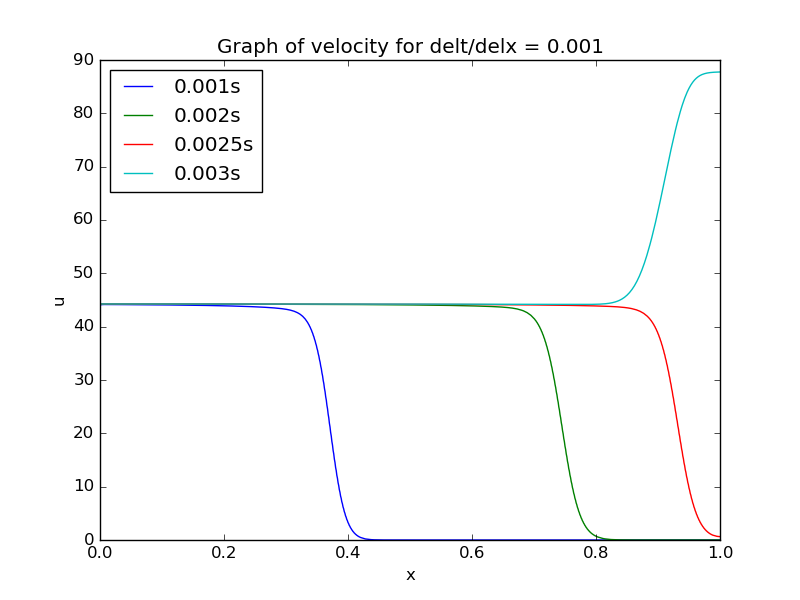
\includegraphics[width = 0.9\textwidth]{lax_fed_3_4.png}
 \caption{Plot of velocity v/s x}
\end{figure}
\begin{figure}[H]
 \centering
 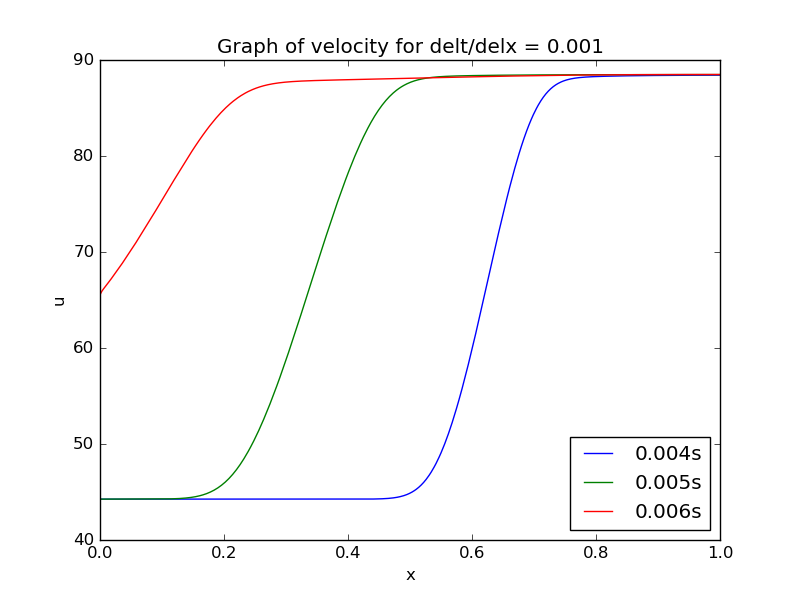
\includegraphics[width = 0.9\textwidth]{lax_fed_3_5.png}
 \caption{Plot of velocity v/s x}
\end{figure}
\begin{figure}[H]
 \centering
 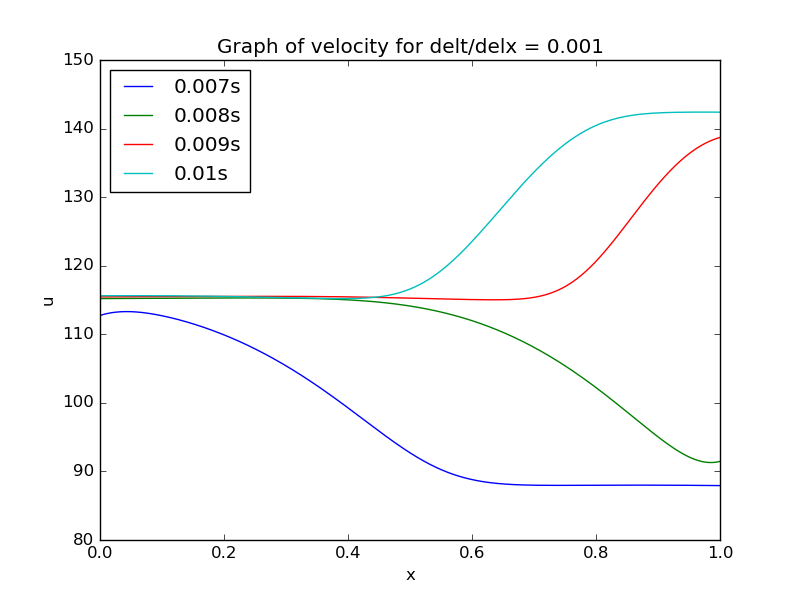
\includegraphics[width = 0.9\textwidth]{lax_fed_3_6.png}
 \caption{Plot of velocity v/s x}
\end{figure}
\begin{figure}[H]
 \centering
 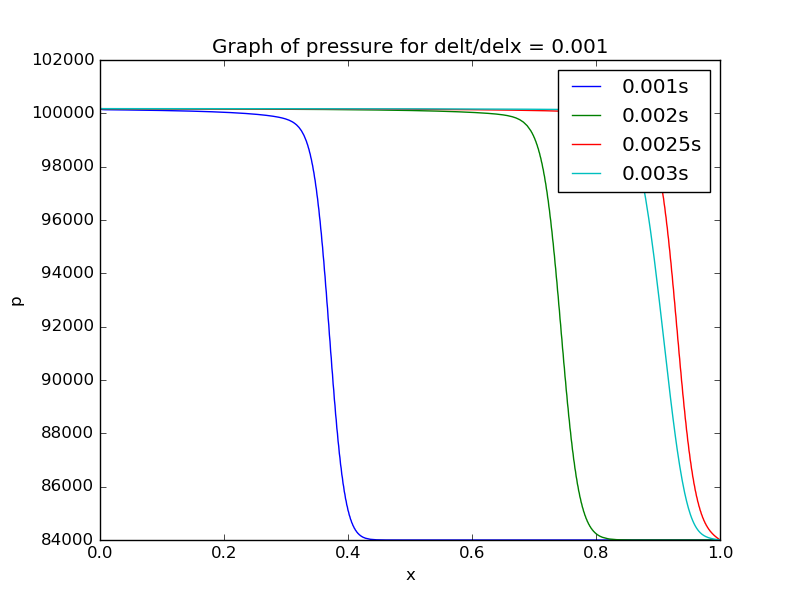
\includegraphics[width = 0.9\textwidth]{lax_fed_3_7.png}
 \caption{Plot of pressure v/s x}
\end{figure}
\begin{figure}[H]
 \centering
 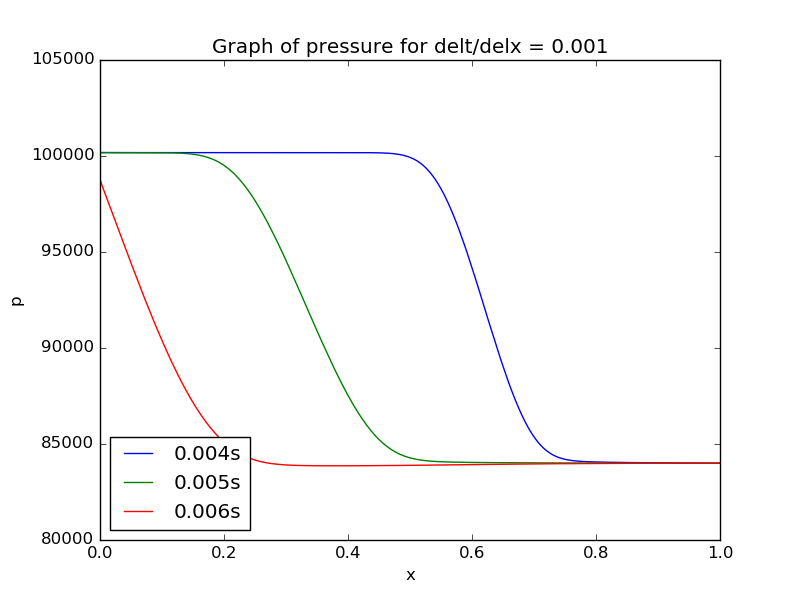
\includegraphics[width = 0.9\textwidth]{lax_fed_3_8.png}
 \caption{Plot of pressure v/s x}
\end{figure}
\begin{figure}[H]
 \centering
 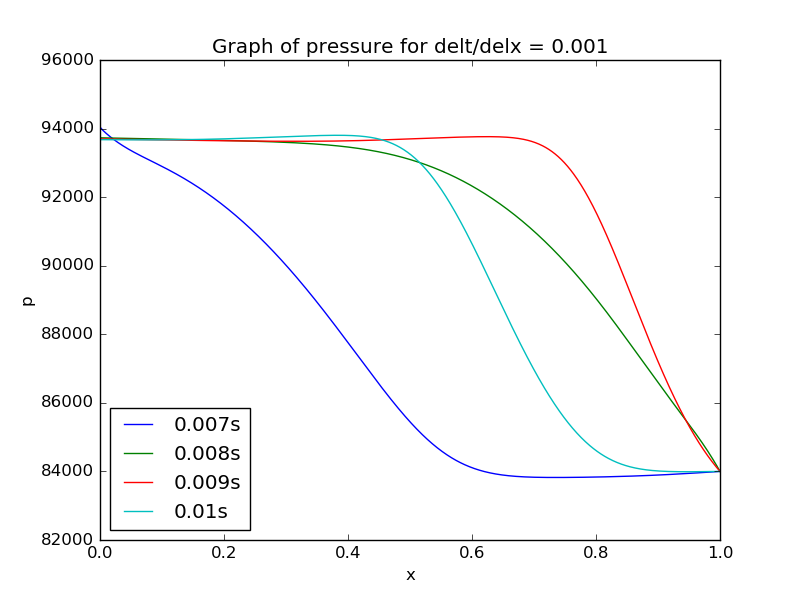
\includegraphics[width = 0.9\textwidth]{lax_fed_3_9.png}
 \caption{Plot of pressure v/s x}
\end{figure}

\subsection{Case 2: $\Delta t = 0.002 \Delta x$}
\begin{figure}[H]
 \centering
 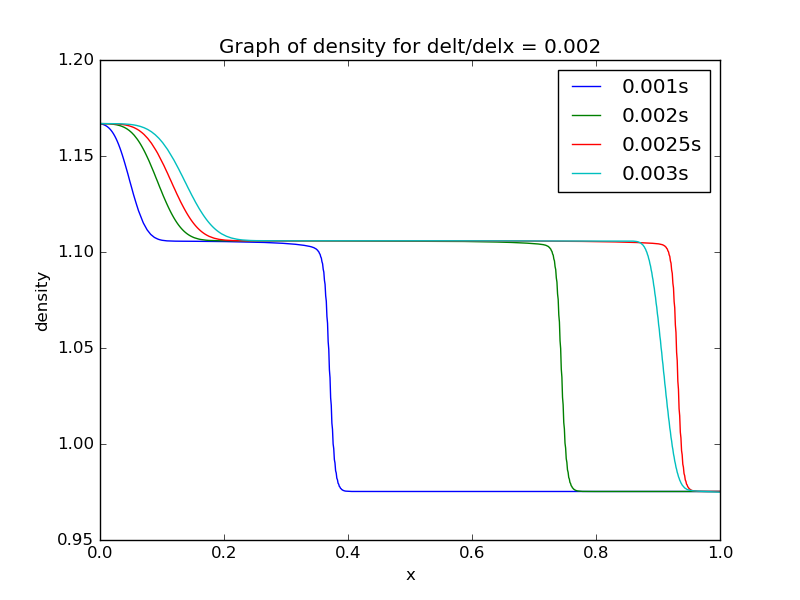
\includegraphics[width = 0.9\textwidth]{lax_fed_4_1.png}
 \caption{Plot of density v/s x}
\end{figure}
\begin{figure}[H]
 \centering
 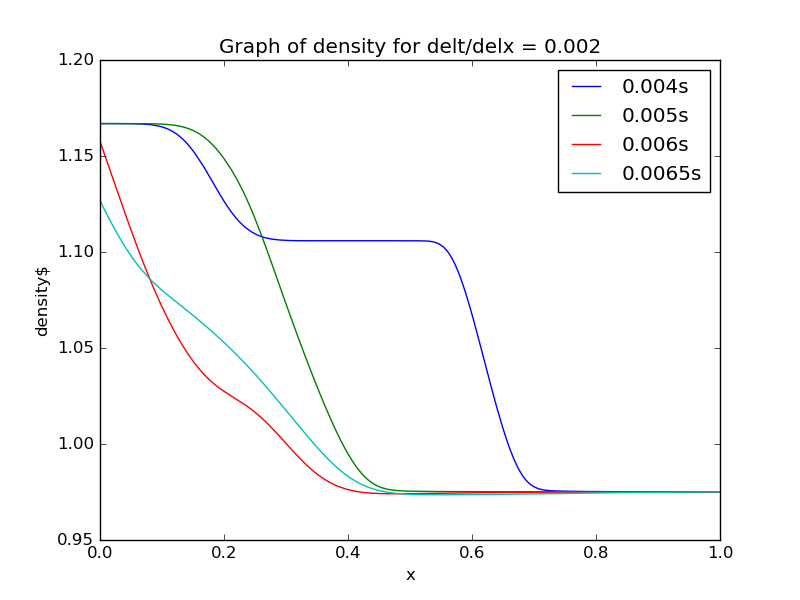
\includegraphics[width = 0.9\textwidth]{lax_fed_4_2.png}
 \caption{Plot of density v/s x}
\end{figure}
\begin{figure}[H]
 \centering
 \includegraphics[width = 0.9\textwidth]{lax_fed_4_3.png}
 \caption{Plot of density v/s x}
\end{figure}
\begin{figure}[H]
 \centering
 \includegraphics[width = 0.9\textwidth]{lax_fed_4_4.png}
 \caption{Plot of velocity v/s x}
\end{figure}
\begin{figure}[H]
 \centering
 \includegraphics[width = 0.9\textwidth]{lax_fed_4_5.png}
 \caption{Plot of velocity v/s x}
\end{figure}
\begin{figure}[H]
 \centering
 \includegraphics[width = 0.9\textwidth]{lax_fed_4_6.png}
 \caption{Plot of velocity v/s x}
\end{figure}
\begin{figure}[H]
 \centering
 \includegraphics[width = 0.9\textwidth]{lax_fed_4_7.png}
 \caption{Plot of pressure v/s x}
\end{figure}
\begin{figure}[H]
 \centering
 \includegraphics[width = 0.9\textwidth]{lax_fed_4_8.png}
 \caption{Plot of pressure v/s x}
\end{figure}
\begin{figure}[H]
 \centering
 \includegraphics[width = 0.9\textwidth]{lax_fed_4_9.png}
 \caption{Plot of pressure v/s x}
\end{figure}

\section{Question 3:}
In this question we solve the Sod's shock tube problem and plot the results at t=0.2. We choose a domain of size 1 and divide 
it into $1000$ grid points implying $\Delta x = 0.001$. The initial conditions are as follows:
\begin{itemize}
 \item \textbf{Left:} $\rho_l, p_l, u_l = 1.0, 1.0, 1.0$
 \item \textbf{Right:} $\rho_r, p_r, u_r = 0.125, 0.1, 0.0$
\end{itemize}
The left and the right half are seperated by diaphragm which is removed at $t = 0.2$. The plot of density, pressure, velocity
and internal energy are shown below

\begin{figure}[H]
 \centering
 \includegraphics[width = 0.9\textwidth]{Sh_tube_den.png}
 \caption{Plot of density v/s x at 0.2s}
\end{figure}

\begin{figure}[H]
 \centering
 \includegraphics[width = 0.9\textwidth]{Sh_tube_vel.png}
 \caption{Plot of velocity v/s x at 0.2s}
\end{figure}

\begin{figure}[H]
 \centering
 \includegraphics[width = 0.9\textwidth]{Sh_tube_p.png}
 \caption{Plot of pressure v/s x at 0.2s}
\end{figure}

\begin{figure}[H]
 \centering
 \includegraphics[width = 0.9\textwidth]{Sh_tube_en.png}
 \caption{Plot of energy v/s x at 0.2s}
\end{figure}

Consider the density plot. We can see that there are three waves, two propogating towards right and one propogating leftwards.
By comparing this with the pressure, velocity and internal energy plot, we see that along the left propogating wave $\rho, 
p, e$ decrease while $u$ increases. Also the change is gradual, implying that this is an expansion fan. Now consider the faster
one among the two waves propogating to the right. We can see that $\rho, u, p, e$ increase downstream of this wave. Thus this 
corresponds to a shock. Along the slower right propogating wave, only $\rho$ and $e$ change implying that this is the contact
surface. Given it is a contact surface it must travel with a speed of $u$. The shock travels with a speed $u + c$ and expansion
fan travels with a speed of $u-c$

\section{Conclusion}
This assignment gives us an insight into the dissipation, dispersion in the FTCS2 and the Lax-Friedrichs schemes. We can say
that the Lax-Friedrichs scheme is more stable than FTCS2 but smoothens the solution. We also see that increasing $\Delta t/
\Delta x$ makes the solution less smooth in both cases i.e higher wave numers are dissipated slower. The animation of how the
properties change is attached along with the assignment for both the cases.
We can see that the solution of the shock matches with the theoretical results and we were able to identify the shock, 
expansion wave and contact surface fromt he plots







\end{document}

